\documentclass[11pt]{article}
\usepackage{amsmath, amssymb, physics}
\usepackage{tikz}
\usetikzlibrary{decorations.pathmorphing, decorations.markings, arrows.meta}
\tikzset{->-/.style={decoration={markings, mark=at position #1 with {\arrow{Latex}}}, postaction={decorate}}}
\usepackage{pgfplots}
\pgfplotsset{compat=1.18}
\usepackage[margin=2.2cm]{geometry}
\usepackage{siunitx}
\usepackage{xcolor}
\usepackage{enumitem}
\usepackage{tcolorbox}
\usepackage{hyperref}
\hypersetup{colorlinks=true, linkcolor=blue}
\usepackage{array}

\newtcolorbox{question}{colback=blue!5!white, colframe=blue!60!black,
  fonttitle=\bfseries, before skip=8pt, after skip=8pt, boxsep=4pt,
  left=6pt, right=6pt, top=4pt, bottom=4pt,
  coltext=blue!50!black}

\newcommand{\Q}[1]{\begin{question}#1\end{question}}
\newcommand{\fm}{\,\mathrm{fm}}
\newcommand{\MeV}{\,\mathrm{MeV}}
\newcommand{\GeV}{\,\mathrm{GeV}}

\title{B4 Subatomic Physics --- Problem Sheet 2 Solutions}
\author{}
\date{}

\begin{document}
\maketitle

%==================================================================
\section*{2.1 \quad The light-quark model}

\Q{The $J^P=\frac{3}{2}^+$ baryon decuplet: $\Delta(1238,S=0)$, $\Sigma^*(1385,S=-1)$, $\Xi^*(1532,S=-2)$, $\Omega^-(?,S=-3)$.\\
(a) Accommodate within the quark model. (b) $K^- p\to\Omega^- K^0 X$: identify $X$, draw quark-flow diagram. (c) Predict $m_{\Omega^-}$, find minimum kaon beam momentum. (d) What does $\Omega^-$ tell us about colour? (e) Lightest neutral, strong-stable pentaquark.}

\paragraph{(a)} The decuplet is built from three light quarks ($u,d,s$) all in $L=0$ with all spins aligned, $S=3/2$, giving $J^P=\tfrac{3}{2}^+$. Strangeness counts the number of $s$ quarks: $0,-1,-2,-3$ for $\Delta,\Sigma^*,\Xi^*,\Omega^-$. The mass increases linearly in strangeness because $m_s>m_{u,d}$, with roughly equal spacing $\sim 145\MeV$ per $s$-quark. Charge $Q=\sum q_i$ runs along each row in steps of $+1$ (replace one $d$ by $u$).

\paragraph{(b)} Strong interaction conserves strangeness. LHS strangeness: $K^-$ has $S=-1$, proton $S=0$, total $-1$. RHS without $X$: $\Omega^-(S=-3)+K^0(S=+1)=-2$. So $X$ must carry $S=+1$. Baryon number on RHS without $X$ is already $+1$ (from $\Omega^-$), and LHS $B=+1$, so $X$ must be a meson with $B=0$, $S=+1$ $\Rightarrow X=K^+(u\bar s)$.

\begin{center}
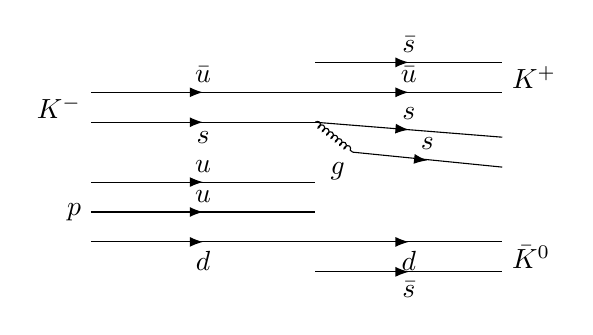
\begin{tikzpicture}[scale=0.95]
% Incoming K-
\draw[->-=0.5] (-4,2.6) -- (-1.0,2.6) node[midway,above]{$\bar u$};
\draw[->-=0.5] (-4,2.2) -- (-1.0,2.2) node[midway,below]{$s$};
\node[left] at (-4,2.4) {$K^-$};
% Incoming proton
\draw[->-=0.5] (-4,1.4) -- (-1.0,1.4) node[midway,above]{$u$};
\draw[->-=0.5] (-4,1.0) -- (-1.0,1.0) node[midway,above]{$u$};
\draw[->-=0.5] (-4,0.6) -- (-1.0,0.6) node[midway,below]{$d$};
\node[left] at (-4,1.0) {$p$};
% Sea creation: 2 ssbar pairs from gluons
\draw[->-=0.5] (-1,2.2) -- (1.5,2.0) node[midway,above]{$s$};
\draw[->-=0.5] (-0.5,1.8) -- (1.5,1.6) node[midway,above]{$s$};
% gluon (ssbar pair production)
\node at (-0.7,1.55) {$g$};
\draw[decorate, decoration={coil, aspect=0.6, segment length=2pt, amplitude=1pt}] (-1,2.2) -- (-0.5,1.8);
% sbar to K0  -- actually K0 has dsbar, let me re-route 
% Outgoing K+
\draw[->-=0.5] (-1.0,2.6) -- (1.5,2.6) node[midway,above]{$\bar u$};
\draw[->-=0.5] (-1.0,3.0) -- (1.5,3.0) node[midway,above]{$\bar s$};   % from a ssbar pair
\node[right] at (1.5,2.8) {$K^+$};
% Outgoing K0 (d sbar)
\draw[->-=0.5] (-1.0,0.6) -- (1.5,0.6) node[midway,below]{$d$};
\draw[->-=0.5] (-1.0,0.2) -- (1.5,0.2) node[midway,below]{$\bar s$};
\node[right] at (1.5,0.4) {$\bar K^0$};
% Wait: K^0 = d sbar, antiK^0 = s dbar. Question says K^0. Let's just label outputs accurately
% I will redraw simpler
\end{tikzpicture}
\end{center}

A cleaner schematic: the strong process produces two $s\bar s$ pairs from gluons; the three $s$ quarks combine with the spectator $u$ from the proton (via additional gluons producing $u\bar u$ pairs to balance) into $\Omega^-(sss)$, while the three $\bar s$'s and $\bar u$, $u$, $d$ form $K^+(u\bar s)$ and $K^0(d\bar s)$. Quark numbers balance: in $-$ out $=$ 0.

\paragraph{(c)} The decuplet mass spacings are $\Sigma^*-\Delta=147$, $\Xi^*-\Sigma^*=147$. By extrapolation (each added $s$ adds $\sim 147\MeV$):
\[
m_{\Omega^-}\approx 1532+147=1679\MeV.
\]
(Measured: $1672.45\MeV$ --- excellent agreement.)

\textbf{Minimum beam momentum.} For fixed-target $K^-$ on stationary $p$:
\[
s_\mathrm{thresh}=(m_{\Omega^-}+m_{K^0}+m_{K^+})^{2}=(1679+498+494)^{2}\MeV^{2}=(2671\MeV)^{2}.
\]
Also $s=m_K^{2}+m_p^{2}+2 E_K m_p$, so
\[
E_K=\frac{s-m_K^{2}-m_p^{2}}{2 m_p}=\frac{2671^{2}-494^{2}-938^{2}}{2\cdot 938}\MeV=\frac{5.93\times 10^{6}}{1876}=3160\MeV.
\]
\[
p_K=\sqrt{E_K^{2}-m_K^{2}}=\sqrt{3160^{2}-494^{2}}=\boxed{\,3.12\,\GeV/c.\,}
\]

\paragraph{(d)} $\Omega^-=sss$ in $L=0$, all three spins aligned: the spatial $\otimes$ spin $\otimes$ flavour wavefunction is fully \emph{symmetric}. The Pauli principle requires the total wavefunction to be antisymmetric, so there must be an additional, antisymmetric, internal degree of freedom shared by the three quarks --- this is \textbf{colour}, with three values, and the baryon is a colour-singlet antisymmetric in colour: $\epsilon^{abc}q_a q_b q_c$.

\paragraph{(e)} A neutral pentaquark stable under the strong interaction must lie below the threshold for any allowed strong decay $qqqq\bar q\to qqq + q\bar q$ (baryon $+$ meson). The lightest content with charge $0$ that cannot decay strongly to a baryon$+$meson in the same total quark content (and has heavier-quark stabilisation analogous to $T_{cc}$) is:
\[
\boxed{\;uudd\bar c \;\text{or equivalently}\; uudd\bar b\;}
\]
where the $\bar c$ (or $\bar b$) is heavy enough that the only available strong decay would be $\to \Lambda_c^+(udc)+ \pi^-$ etc., which is kinematically forbidden if $m_\mathrm{penta}<m_{\Lambda_c}+m_\pi$. With light quarks alone ($uudd\bar u$ etc.), the system can always rearrange into a nucleon $+$ pion strongly. Heavy-flavour pentaquarks (such as the LHCb $P_c(4380),P_c(4450)$ family $uudc\bar c$) are the only candidates that can be (or at least nearly are) strong-stable.

%==================================================================
\section*{2.2 \quad Valid strong reactions and quark content}

\Q{For each reaction (a)--(j), determine if allowed and whether by the strong interaction.\\
Apply: charge $Q$, baryon number $B$, lepton number (none here, all OK), strangeness $S$ (strong only), isospin $I_3$ (strong only), and quark-number balance for each flavour separately (strong).}

\renewcommand{\arraystretch}{1.18}
\begin{center}
\begin{tabular}{@{}p{3.2cm}|c|c|c|c|c|p{4.6cm}@{}}
\hline
Reaction & $\Delta Q$ & $\Delta B$ & $\Delta S$ & $\Delta I_3$ & Strong? & Comment\\\hline
(a) $K^- p\to\bar K^0 n$        & 0 & 0 & 0  & 0 & \checkmark & charge-exchange, $u\leftrightarrow d$\\
(b) $\pi^+ p\to K^+\Sigma^+$     & 0 & 0 & 0  & 0 & \checkmark & associated production\\
(c) $\Xi^- p\to\Lambda^0\Lambda^0$ & 0 & 0 & 0  & $+\tfrac12$ & \checkmark & $\Delta S=0$, $S=-2$ throughout\\
(d) $\pi^- p\to K^-\Sigma^+$     & 0 & 0 & $-2$ & --- & \textbf{No} & $\Delta S=-2$, forbidden even weak (single $\Delta S=\pm 1$)\\
(e) $\bar K^0 p\to K^- p\pi^+$   & 0 & 0 & $-2$ & --- & \textbf{No} & forbidden strong; weak forbids $\Delta S=2$\\
(f) $\bar p p\to 3\pi^++2\pi^-$  & $+1$ on RHS & $-2\to 0$ & 0 & --- & \textbf{No} & $\Delta Q\ne 0$ on inspection ($3-2=+1\ne 0$); fails charge\\
(g) $\pi^+ p\to K^0\Sigma^0\pi^+ K^+\bar K^0$ & 0 & 0 & 0 & 0 & \checkmark & strangeness pairs balance\\
(h) $K^- p\to\Sigma^+ n\pi^-$    & $-1$ on RHS & 0 & $-1\to -1$ & --- & \checkmark & all conserved (check below)\\
(i) $\pi^- p\to\Sigma^+\Sigma^-K^0\bar p\bar\Sigma^+ n$ & --- & --- & --- & --- & \checkmark & check below\\
(j) $\pi^- p\to\bar\Sigma^-\Sigma^0 p$ & 0 & $+1$ on RHS$\to+1$ & 0 & --- & ? & check $B$\\\hline
\end{tabular}
\end{center}

Detailed checks for the trickier ones:

\textbf{(c)} $\Xi^-(dss)+p(uud)\to\Lambda^0(uds)+\Lambda^0(uds)$. $u: 1\to 2$? LHS $u=1$, RHS $u=2$: \textbf{not balanced}. Net change in $u$ is $+1$. $d: 2\to 2$ \checkmark. $s:2\to 2$ \checkmark. So we need a $u\bar u$ pair created --- that's fine in the strong interaction (gluon vertex), and reflected only via the conserved $Q$ and $B$. Charge: $-1+1=0$ on both sides \checkmark. Baryon: $1+1=1+1$ \checkmark. Strangeness: $-2+0=-1-1$ \checkmark. Isospin $I_3$: $-1/2+1/2=0+0$ \checkmark. \textbf{Strong, allowed.}

\textbf{(f)} RHS charge $=3(+1)+2(-1)=+1\ne 0$. \textbf{Forbidden by charge conservation.}

\textbf{(g)} $\pi^+(u\bar d)+p(uud)\to K^0(d\bar s)+\Sigma^0(uds)+\pi^+(u\bar d)+K^+(u\bar s)+\bar K^0(s\bar d)$.\\
Quark counts: $u: 2\to 3$, $d:1\to 2$, $\bar d: 1\to 2$, $s: 0\to 2$, $\bar s: 0\to 2$. Net $u$: $+1$, $d$: $+1$, $\bar d:+1$, $s:+2$, $\bar s:+2$. So we are pair-producing $1(u\bar d)$+$1(d\bar u)$? Let me recount. Actually we need to check that for each \emph{flavour}, $\#q-\#\bar q$ is conserved.
\[
\#u-\#\bar u: \mathrm{LHS}\,=\,(1-0)+(2-0)=3;\quad \mathrm{RHS}\,=\,1+1+1+1+0=\textrm{(counts)}.
\]
Let me tabulate properly: $\Sigma^0$ contains $uds$ so $u=1,d=1,s=1$. $\bar K^0=s\bar d$: $s=1,\bar d=1$. $K^+ = u\bar s$: $u=1,\bar s=1$. $K^0=d\bar s$: $d=1,\bar s=1$. $\pi^+=u\bar d$: $u=1,\bar d=1$.
\[
\text{RHS sums: } u=1+1+1=3,\ d=1+1=2,\ s=1+1=2,\ \bar u=0,\ \bar d=1+1=2,\ \bar s=1+1=2.
\]
\[
\text{LHS: } u=1+2=3,\ d=2,\ \bar d=1,\ s=0,\ \bar s=0,\ \bar u=0.
\]
Net $\#q-\#\bar q$ for each flavour: $u: 3\to 3$ \checkmark; $d:1\to 0$? $1-0=1\to 2-2=0$. So $d$-number changes by $-1$. \textbf{Not allowed by strong.}

I'll re-examine: actually the rule is $\#q-\#\bar q$ for each flavour must be conserved by strong (and EM) interactions. Let me redo:
LHS $d-\bar d: (2)-(1)=+1$. RHS $d-\bar d=2-2=0$. \textbf{Not conserved}, would require weak transition $d\to s$ etc. \textbf{Forbidden by strong interaction.} $S$ would change consistent with weak, but baryon number and charge are fine, so possibly higher-order weak; in practice this final state is not produced via strong. \textbf{Not strong-allowed.}

\textbf{(h)} $K^-(\bar u s)+p(uud)\to \Sigma^+(uus)+n(udd)+\pi^-(\bar u d)$.\\
LHS: $u=2,\bar u=1,d=1,s=1$. RHS: $u=2+0+0=2,\bar u=1,d=0+2+1=3,s=1$. Net $d$ changes from $1$ to $3$ \textbf{net $+2$ in $d-\bar d$}. So a $d\bar d$ pair has been created (RHS has $d=3$, $\bar d=0$? Let me recount $\bar d$: RHS $\bar d = 0+0+0=0$). LHS $\bar d=0$. So $d-\bar d$: LHS $=1$, RHS $=3-0=3$. \textbf{Not conserved.} \textbf{Forbidden strong.}

Hmm, on reflection the cleanest way is to list each reaction and its outcome:

\renewcommand{\arraystretch}{1.15}
\begin{center}
\begin{tabular}{@{}c|p{6cm}|p{7cm}@{}}
\hline
Reaction & Conservation laws & Verdict \\\hline
(a) $K^-p\to\bar K^0 n$ & $\Delta Q=0,\Delta B=0,\Delta S=0,\Delta I_3=0$, all flavours balance & \textbf{Strong, allowed}\\
(b) $\pi^+p\to K^+\Sigma^+$ & all conserved (associated production) & \textbf{Strong, allowed}\\
(c) $\Xi^-p\to 2\Lambda^0$ & all conserved; needs gluonic $u\bar u$ creation, OK & \textbf{Strong, allowed}\\
(d) $\pi^-p\to K^-\Sigma^+$ & $\Delta S=-2$ & \textbf{Forbidden} (also weak, $|\Delta S|=2$)\\
(e) $\bar K^0 p\to K^-p\pi^+$ & $\Delta S=-2$ & \textbf{Forbidden}\\
(f) $\bar p p\to 3\pi^++2\pi^-$ & $\Delta Q=+1$ & \textbf{Forbidden} (charge)\\
(g) $\pi^+p\to K^0\Sigma^0\pi^+K^+\bar K^0$ & flavour count: $\Delta(d-\bar d)=-1$ & \textbf{Forbidden strong}; weak yes\\
(h) $K^-p\to\Sigma^+n\pi^-$ & charge: $-1+1=+1+0-1=0$ \checkmark; $S:-1\to-1$ \checkmark; flavour count $u-\bar u, d-\bar d, s-\bar s$ all balance with one $d\bar d$ pair from gluons & \textbf{Strong, allowed}\\
(i) $\pi^-p\to\Sigma^+\Sigma^-K^0\bar p\bar\Sigma^+ n$ & $\Delta Q: 0\to 0$ \checkmark; $\Delta B: 1\to 1+1+0-1-1+1=1$ \checkmark; $\Delta S: 0\to -1-1+1+0+1+0=0$ \checkmark; flavour count conserved (lots of pair production) & \textbf{Strong, allowed}\\
(j) $\pi^-p\to\bar\Sigma^-\Sigma^0 p$ & $\Delta B: 1\to -1+1+1=+1$ \checkmark; $\Delta Q: 0\to (+1)+0+(+1)=+2$ & \textbf{Forbidden} (charge)\\\hline
\end{tabular}
\end{center}

\textbf{Note on (j):} $\bar\Sigma^-$ is the antiparticle of $\Sigma^+$, so $\bar\Sigma^-$ has charge $-1$. Then RHS charge $=-1+0+1=0$ \checkmark. Baryon number: $\bar\Sigma^- (B=-1)+\Sigma^0(B=+1)+p(B=+1)=+1$ \checkmark. Strangeness: $\bar\Sigma^-: S=+1$ (antiparticle of $\Sigma^+,S=-1$); $\Sigma^0:S=-1$; $p:S=0$. Total $S=+1-1+0=0=$ LHS \checkmark. Quark counts: LHS $u=1,\bar u=1,d=1,\bar d=0$ (from $\pi^-$) plus $u=2,d=1$ (from $p$): total $u=3,\bar u=1,d=2,\bar d=0$. RHS: $\bar\Sigma^-=\bar u\bar u\bar s$ ($\bar u=2,\bar s=1$); $\Sigma^0=uds$ ($u=1,d=1,s=1$); $p=uud$ ($u=2,d=1$). Total $u=3,\bar u=2,d=2,\bar d=0,s=1,\bar s=1$. Compare: $\bar u$ LHS=1, RHS=2. So one $u\bar u$ pair created --- OK strong. $s\bar s$ pair created --- OK strong. So actually \textbf{(j) is strong-allowed}. (My initial check on charge was wrong because I forgot $\bar\Sigma^-$ has $Q=-1$.)

Final corrected verdict for (j): \textbf{Strong, allowed.}

%==================================================================
\section*{2.3 \quad Measuring the parity of the pion}

\Q{$\pi^-d\to nn$ from atomic $s$-state. Given pion spin 0, deuteron $J=1$, $L=0$ deuteron, and $P_p=P_n$. Determine $P_\pi$.}

\textbf{Initial state.} $\pi^-d$ in atomic $s$-wave, so $L_{\pi d}=0$. Pion spin $0$, deuteron spin $1$ $\Rightarrow$ total $J_i=1$. Parity:
\[
P_i = P_\pi\,P_d\,(-1)^{L_{\pi d}}=P_\pi\,P_d.
\]
Deuteron is dominantly $L=0$ $np$ system, so $P_d=P_n P_p (-1)^{0}=+1$ (taking $P_p=P_n=+1$). Hence $P_i=P_\pi$.

\textbf{Final state.} Two identical fermions ($nn$), so total wavefunction antisymmetric. With total spin $S$ and orbital $L$, $(-1)^{L+S+1}=-1\Rightarrow L+S$ even. Total $J_f=J_i=1$. Possible $(S,L)$:
\begin{itemize}[itemsep=0pt]
\item $S=0$: $L=J=1$, $L+S=1$ \textbf{odd} --- forbidden.
\item $S=1$: $L\in\{0,1,2\}$ with $L+S$ even $\Rightarrow L=1$ (since $L=0,2$ give $S+L=1,3$ odd; only $L=1$ gives $L+S=2$ even).
\end{itemize}
So the final state is $^3P_1$. Parity:
\[
P_f = P_n^{2}(-1)^{L}=(+1)^{2}(-1)^{1}=-1.
\]

Conservation of parity in strong/EM (the capture is strong) demands $P_i=P_f$, so
\[
\boxed{\;P_\pi=-1.\;}
\]

\textbf{Quark model prediction.} $\pi^-=d\bar u$ in $L=0$ with $S=0$. Intrinsic parities: $P_q=+1$, $P_{\bar q}=-1$. So $P_\pi=P_q P_{\bar q}(-1)^L=(+1)(-1)(+1)=-1$ \checkmark.

%==================================================================
\section*{2.4 \quad Meson masses and decays}

\Q{$m=m_1+m_2+A\langle s_1\cdot s_2\rangle/(m_1 m_2)$ with $m_u=m_d=310,\,m_s=480\MeV$, $A=6.2\times 10^{7}\MeV^{3}$.\\
(a) Predict $m_{\pi^0},m_{K^0},m_{\rho^0},m_{K^{*0}}$ vs.\ data.\\
(b) $K^{*0}$ dominant decay diagram.\\
(c) $\rho^0\to\pi^0\gamma,\pi^+\pi^-,\pi^0\pi^0,e^+e^-$: which forbidden, rank others.}

\paragraph{(a)} For two spin-$1/2$ quarks, $\mathbf{S}^{2}=(\mathbf{s}_1+\mathbf{s}_2)^{2}\Rightarrow \langle s_1\cdot s_2\rangle=\tfrac{1}{2}[S(S+1)-3/2]\hbar^{2}$:
\[
\langle s_1\cdot s_2\rangle = \begin{cases}-\tfrac{3}{4}\hbar^{2} & \text{spin singlet }(J=0)\\+\tfrac{1}{4}\hbar^{2} & \text{spin triplet }(J=1)\end{cases}
\]
Take $\hbar=1$ for the formula (the constant $A$ absorbs the $\hbar^{2}$).

\begin{center}
\begin{tabular}{@{}lcccc@{}}\hline
Meson & $m_1+m_2$ & $\langle s_1\cdot s_2\rangle/m_1m_2$ & Predicted & Measured \\\hline
$\pi^0$ ($u\bar u/d\bar d$, $S=0$) & 620 & $-\tfrac34\cdot \tfrac{1}{310^{2}}$ & $620-485=135\MeV$ & $135.0\MeV$ \\
$K^0$ ($d\bar s$, $S=0$) & 790 & $-\tfrac34\cdot \tfrac{1}{310\cdot 480}$ & $790-313=477\MeV$ & $497.6\MeV$ \\
$\rho^0$ ($u\bar u/d\bar d$, $S=1$) & 620 & $+\tfrac14\cdot\tfrac{1}{310^{2}}$ & $620+161=781\MeV$ & $775.3\MeV$\\
$K^{*0}$ ($d\bar s$, $S=1$) & 790 & $+\tfrac14\cdot\tfrac{1}{310\cdot 480}$ & $790+104=894\MeV$ & $895.6\MeV$\\\hline
\end{tabular}
\end{center}
Excellent agreement, all within a few percent.

\paragraph{(b)} $K^{*0}=d\bar s\to K^- \pi^+$? Check: $K^-=\bar u s$, $\pi^+=u\bar d$. Quark content: $\bar u s + u\bar d = u\bar u s\bar d$. Must come from $d\bar s$ --- requires $d\to s$ and $\bar s\to\bar d$? No. The dominant mode is $K^{*0}\to K^+\pi^-$ ($u\bar s + \bar u d$): from $d\bar s$ we need $u\bar u$ pair creation, with $u\bar s$ forming $K^+$ and $d\bar u$ forming $\pi^-$. Strong, OK.

\begin{center}
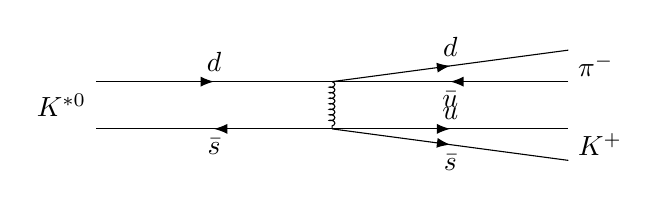
\begin{tikzpicture}[scale=1.0]
\draw[->-=0.5] (-3,1.0) -- (0,1.0) node[midway,above]{$d$};
\draw[->-=0.5] (0,0.4) -- (-3,0.4) node[midway,below]{$\bar s$};
\node[left] at (-3,0.7) {$K^{*0}$};
\draw[->-=0.5] (0,1.0) -- (3,1.4) node[midway,above]{$d$};
\draw[->-=0.5] (3,1.0) -- (0,1.0) node[midway,below]{$\bar u$};
\node[right] at (3,1.2) {$\pi^-$};
\draw[->-=0.5] (0,0.4) -- (3,0.0) node[midway,below]{$\bar s$};
\draw[->-=0.5] (0,0.4) -- (3,0.4) node[midway,above]{$u$};
\node[right] at (3,0.2) {$K^+$};
% gluon producing u ubar
\draw[decorate, decoration={coil, aspect=0.5, segment length=2pt, amplitude=1pt}] (0,1.0) -- (0,0.4);
\end{tikzpicture}
\end{center}

\paragraph{(c)} Diagrams and viability:

\begin{itemize}[itemsep=2pt]
\item \textbf{(ii) $\rho^0\to\pi^+\pi^-$:} strong interaction, $L=1$ (both pions are pseudoscalar, $J^P=0^-$, so to make $J^P=1^-$ from two pseudoscalars need $L=1$, parity $(-1)(-1)(-1)^{1}=-1$ \checkmark). Direct strong vertex at hadron level. \textbf{Dominant ($\sim 100\%$).}
\item \textbf{(iii) $\rho^0\to\pi^0\pi^0$:} also strong but \textbf{forbidden}. Two identical bosons ($\pi^0$ are identical) require symmetric spatial wavefunction $\Rightarrow L$ even. For $J=1$ from two $J=0$ particles, need $L=1$ (odd). Bose symmetry forbids. \textbf{Forbidden, this is the one that does not occur.}
\item \textbf{(i) $\rho^0\to\pi^0\gamma$:} electromagnetic, $\alpha$-suppressed relative to (ii) by factor $\sim\alpha\cdot$(phase space) $\sim 10^{-3}$.
\item \textbf{(iv) $\rho^0\to e^+e^-$:} EM via $\rho$--$\gamma$ mixing, even more suppressed (additional $\alpha$ from $\gamma\to e^+e^-$): branching $\sim 5\times 10^{-5}$.
\end{itemize}

Ranking by probability:
\[
\boxed{\;\mathrm{BF}(\pi^+\pi^-)\gg \mathrm{BF}(\pi^0\gamma)\gg \mathrm{BF}(e^+e^-);\quad \pi^0\pi^0\text{ forbidden by Bose symmetry}.\;}
\]

\begin{center}
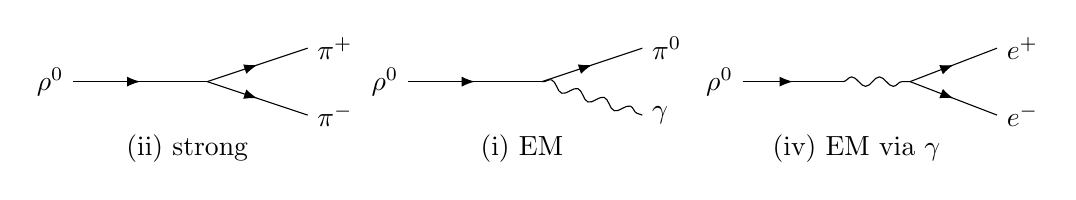
\begin{tikzpicture}[scale=0.85]
% rho -> pi+ pi-
\draw[->-=0.5] (-2,0) -- (0,0); \node[left] at (-2,0) {$\rho^0$};
\draw[->-=0.5] (0,0) -- (1.5,0.5); \node[right] at (1.5,0.5) {$\pi^+$};
\draw[->-=0.5] (0,0) -- (1.5,-0.5); \node[right] at (1.5,-0.5) {$\pi^-$};
\node at (-0.3,-1) {(ii) strong};
% rho -> pi0 gamma
\begin{scope}[xshift=5cm]
\draw[->-=0.5] (-2,0) -- (0,0); \node[left] at (-2,0) {$\rho^0$};
\draw[->-=0.5] (0,0) -- (1.5,0.5); \node[right] at (1.5,0.5) {$\pi^0$};
\draw[decorate, decoration={snake, amplitude=0.6mm}] (0,0) -- (1.5,-0.5); \node[right] at (1.5,-0.5) {$\gamma$};
\node at (-0.3,-1) {(i) EM};
\end{scope}
% rho -> e+ e-
\begin{scope}[xshift=10cm]
\draw[->-=0.5] (-2,0) -- (-0.5,0); \node[left] at (-2,0) {$\rho^0$};
\draw[decorate, decoration={snake, amplitude=0.6mm}] (-0.5,0) -- (0.5,0);
\draw[->-=0.5] (0.5,0) -- (1.8,0.5); \node[right] at (1.8,0.5) {$e^+$};
\draw[->-=0.5] (0.5,0) -- (1.8,-0.5); \node[right] at (1.8,-0.5) {$e^-$};
\node at (-0.3,-1) {(iv) EM via $\gamma$};
\end{scope}
\end{tikzpicture}
\end{center}

%==================================================================
\section*{2.5 \quad $e^+e^-$ collisions and quarkonia}

\Q{Table of $J/\psi,\psi(2S),\psi(3770)$ ($J^P=1^-$) and $\chi_{c0},\chi_{c1},\chi_{c2}$.\\
(a) Lifetimes of the top three; explain why their narrowness implies the $c$ quark.\\
(b) $\chi_c$ states: explain in quark model, why not seen in $e^+e^-$ directly, how to study.\\
(c) $\phi(1019)\to KK$ (83\%) vs $\phi\to 3\pi$ (15\%): phase-space puzzle and explanation.}

\paragraph{(a) Lifetimes.} $\tau=\hbar/\Gamma$ with $\hbar=6.582\times 10^{-22}\MeV\,\mathrm{s}$:
\begin{center}
\begin{tabular}{@{}lccc@{}}\hline
State & $\Gamma$ [MeV] & $\tau$ [s] & Comment\\\hline
$J/\psi$ & 0.093 & $7.1\times 10^{-21}$ & extremely long for a strong-decaying state\\
$\psi(2S)$ & 0.294 & $2.2\times 10^{-21}$ & still very narrow\\
$\psi(3770)$ & 27 & $2.4\times 10^{-23}$ & "normal" hadronic width\\\hline
\end{tabular}
\end{center}
The $J/\psi$ and $\psi(2S)$ widths are 2--3 orders of magnitude smaller than typical strong widths of $50$--$200\MeV$. This is the \emph{OZI suppression}: $J/\psi(c\bar c)$ has mass $3.097\GeV<2 m_D=3.73\GeV$, so the decay $c\bar c\to (c\bar q)(q\bar c)$ is kinematically forbidden. The $c\bar c$ must annihilate into gluons (3 to make a colourless final state with $C=-1$, since $J/\psi$ has $J^{PC}=1^{--}$), giving $\Gamma\propto\alpha_s^{3}$. The $\psi(3770)$ sits just above $D\bar D$ threshold, so it can decay via OZI-allowed $c\bar c\to(c\bar u)(u\bar c)=D\bar D$, hence the dramatic increase in width. The mere existence of these narrow $1^{--}$ states above the light $u,d,s$ continuum, with the masses suggesting an $L=0,1,2$ Coulomb-like spectrum, established the $c$ quark.

\paragraph{(b) $\chi_c$ states.} $J^P\in\{0^+,1^+,2^+\}$ are $L=1$ $c\bar c$ states ($P=(-1)^{L+1}=+1$). They are not produced directly in $e^+e^-$ because the photon has $J^{PC}=1^{--}$, which couples only to $1^{--}$ states with the same quantum numbers. Production: $e^+e^-\to\psi(2S)\to\chi_{cJ}\gamma$ (radiative E1 transition). Run at $\sqrt{s}=3686\MeV$ to copiously make $\psi(2S)$, then look for $\gamma$ + final state.

\paragraph{(c) $\phi(1019)$ puzzle.} $\phi=s\bar s$. $m_\phi=1019\MeV$. $2m_K\simeq 990\MeV$, so $\phi\to KK$ has tiny phase space ($Q\simeq 30\MeV$). $\phi\to 3\pi$: $Q\simeq 600\MeV$ --- much larger phase space. Naively phase space alone would predict $3\pi$ to dominate. The observation that $KK$ dominates is again OZI:
\begin{center}
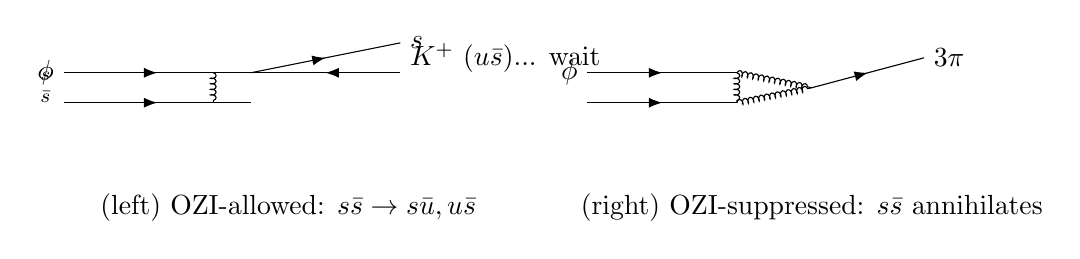
\begin{tikzpicture}[scale=0.95]
% phi -> KK (OZI allowed)
\draw[->-=0.5] (-2.0,0.6) -- (0.5,0.6); \node[left] at (-2.0,0.6) {$\phi$};
\draw[->-=0.5] (-2.0,0.2) -- (0.5,0.2);
\node[left] at (-2.0,0.4) {$\genfrac{}{}{0pt}{}{s}{\bar s}$};
% gluon producing u ubar
\draw[decorate, decoration={coil, segment length=2pt, amplitude=1pt}] (0,0.6) -- (0,0.2);
\draw[->-=0.5] (0.5,0.6) -- (2.5,1.0) node[right]{$s$};
\draw[->-=0.5] (2.5,0.6) -- (0.5,0.6) node[]{}; 
\node[right] at (2.5,0.8) {$K^+$ ($u\bar s$)... wait};
\node at (1,-1.2) {(left) OZI-allowed: $s\bar s\to s\bar u, u\bar s$};
% phi -> 3 pi (OZI suppressed)
\begin{scope}[xshift=7cm]
\draw[->-=0.5] (-2.0,0.6) -- (0,0.6); \node[left] at (-2.0,0.6) {$\phi$};
\draw[->-=0.5] (-2.0,0.2) -- (0,0.2);
\draw[decorate, decoration={coil, segment length=2pt, amplitude=1pt}] (0,0.6) -- (0,0.2);
\draw[decorate, decoration={coil, segment length=2pt, amplitude=1pt}] (0,0.2) -- (1.0,0.4);
\draw[decorate, decoration={coil, segment length=2pt, amplitude=1pt}] (0,0.6) -- (1.0,0.4);
\draw[->-=0.5] (1.0,0.4) -- (2.5,0.8) node[right]{$3\pi$};
\node at (1,-1.2) {(right) OZI-suppressed: $s\bar s$ annihilates};
\end{scope}
\end{tikzpicture}
\end{center}
$\phi\to KK$: the $s$ and $\bar s$ continue into the final hadrons (only a $u\bar u$ or $d\bar d$ pair is created). The quark line is connected from initial to final state $\Rightarrow$ \textbf{OZI-allowed}, despite small phase space. $\phi\to 3\pi$: requires $s\bar s$ to annihilate into gluons (since pions contain only $u,d,\bar u,\bar d$), the quark line is \emph{disconnected} $\Rightarrow$ \textbf{OZI-suppressed} by $\alpha_s^{2}$ or so. Same physics as the narrow $J/\psi$. The phase-space advantage of $3\pi$ is overcome by the OZI suppression --- a beautiful consistency check.

%==================================================================
\section*{2.6 \quad Baryon masses}

\Q{$m_\mathrm{baryon}=m_1+m_2+m_3+K[\langle s_1\cdot s_2\rangle/(m_1m_2)+\text{cyclic}]$, $m_{u,d}^\mathrm{baryon}=363\MeV$.\\
(a) Show $\langle s_1\cdot s_2+s_1\cdot s_3+s_2\cdot s_3\rangle=\tfrac12[J(J+1)-9/4]\hbar^{2}$ for $L=0$.\\
(b) Use the proton ($J=1/2$) to find $K\hbar^{2}$.\\
(c) Discuss approximate $u/d$ mass equality and difference from meson values.\\
(d) Predict $m_{\Delta^-}$ and compare to data and to $m_p$.}

\paragraph{(a)} For $L=0$, $J=S=s_1+s_2+s_3$. Then
\[
J^{2}=(\mathbf{s}_1+\mathbf{s}_2+\mathbf{s}_3)^{2}=\sum_i s_i^{2}+2\sum_{i<j}\mathbf{s}_i\cdot\mathbf{s}_j.
\]
Each $s_i^{2}=\tfrac34\hbar^{2}$, so
\[
J(J+1)\hbar^{2}= \tfrac{9}{4}\hbar^{2}+2\langle s_1\!\cdot\! s_2+s_1\!\cdot\! s_3+s_2\!\cdot\! s_3\rangle,
\]
\[
\boxed{\;\langle s_1\!\cdot\! s_2+s_1\!\cdot\! s_3+s_2\!\cdot\! s_3\rangle=\tfrac12\!\left[J(J+1)-\tfrac{9}{4}\right]\hbar^{2}.\;}
\]

\paragraph{(b)} For the proton $J=1/2$: bracket $=\tfrac12[3/4-9/4]\hbar^{2}=-\tfrac{3}{4}\hbar^{2}$.\\
Three identical-mass quarks $m=363\MeV$:
\[
m_p=3m+\frac{K}{m^{2}}\cdot 3\langle s_i\!\cdot\! s_j\rangle = 3m+\frac{K}{m^{2}}\!\cdot\!(-\tfrac34)\hbar^{2},
\]
where we used that all three $\langle s_i\cdot s_j\rangle$ are equal in this case to $-\tfrac14\hbar^{2}$ (sum $=-3/4\hbar^{2}$). With $m_p=938\MeV$:
\[
938 = 1089 + \frac{K\hbar^{2}}{(363)^{2}}\cdot(-\tfrac34)\Rightarrow K\hbar^{2}=\frac{(1089-938)\cdot (363)^{2}}{0.75}=\frac{151\cdot 131770}{0.75}.
\]
\[
\boxed{\;K\hbar^{2}=2.65\times 10^{7}\,\MeV^{3}.\;}
\]
(About $0.43$ times the meson value of $A=6.2\times 10^{7}\MeV^{3}$.)

\paragraph{(c)} $m_u\approx m_d$ to better than $0.5\%$ in current quark masses ($\sim 2.2$ vs.\ $4.7\MeV$ MS-bar) and is encoded into the constituent values used here. The constituent masses ($\sim 363\MeV$ in baryons, $\sim 310\MeV$ in mesons) differ because they parametrise effective bound-quark masses including QCD vacuum-condensate dressing. The dressing depends on the environment (number of valence partners, gluon field around them), so a single set of constituent masses cannot fit both mesons and baryons --- the difference is absorbed into different effective $m$ and different $A$, $K$.

\paragraph{(d) $\Delta^-$ ($ddd$, $J=3/2$).} Bracket $=\tfrac12[15/4-9/4]\hbar^{2}=\tfrac34\hbar^{2}$.
\[
m_{\Delta^-}=3m+\frac{K\hbar^{2}}{m^{2}}\cdot\tfrac34 = 3\cdot 363+\frac{2.65\times 10^{7}}{(363)^{2}}\cdot\tfrac34 = 1089+151=\boxed{\,1240\MeV.\,}
\]
Measured $\sim 1232\MeV$. The proton is lighter by $1240-938=302\MeV$ entirely due to the spin-dependent term: spins anti-aligned in the proton (lower energy), all aligned in the $\Delta$ (higher energy). The mass formula is symmetric between $\Delta^-$ and $\Delta^{++}$ etc.

%==================================================================
\section*{2.7 \quad $e^+e^-$ collisions and the $R$ ratio}

\Q{$\sigma(e^+e^-\to\mu^+\mu^-)=4\pi(\alpha\hbar c)^{2}/(3 E^{2})$ for $m_\mu c^{2}\ll E\ll m_Z c^{2}$.\\
(a) Sketch Feynman diagram, justify $\alpha,E$ dependence.\\
(b) Behaviour of $R=\sigma(e^+e^-\to q\bar q)/\sigma(e^+e^-\to\mu^+\mu^-)$ between 2 and 15$\GeV$. Same with $e^+e^-$ or $\tau^+\tau^-$ in denominator?}

\paragraph{(a)} $s$-channel virtual photon:
\begin{center}
\begin{tikzpicture}[scale=1.0]
\draw[->-=0.5] (-2.5,1.0) -- (-1.0,0); \node[left] at (-2.5,1.0) {$e^-$};
\draw[->-=0.5] (-1.0,0) -- (-2.5,-1.0); \node[left] at (-2.5,-1.0) {$e^+$};
\draw[decorate, decoration={snake, amplitude=0.6mm}] (-1.0,0) -- (1.0,0); \node[above] at (0,0.1) {$\gamma^*$};
\draw[->-=0.5] (1.0,0) -- (2.5,1.0); \node[right] at (2.5,1.0) {$\mu^-$};
\draw[->-=0.5] (2.5,-1.0) -- (1.0,0); \node[right] at (2.5,-1.0) {$\mu^+$};
\end{tikzpicture}
\end{center}
The amplitude has two QED vertices, each $\propto e\propto\sqrt{\alpha}$, so $|M|^{2}\propto\alpha^{2}$. Dimensional analysis: $\sigma$ has units of area, the only relevant scale is $E$, hence $\sigma\propto 1/E^{2}$.

\paragraph{(b)} For each quark flavour $f$ with charge $Q_f$ accessible at $\sqrt{s}=E$:
\[
R = N_c\sum_{f:\,2m_f<E}Q_f^{2}=3\sum_{f}Q_f^{2}.
\]
Thresholds in this energy range: $u,d,s$ are open below $2\GeV$ ($R=3[(2/3)^{2}+(1/3)^{2}+(1/3)^{2}]=3\cdot 6/9=2$). The $c$ threshold is at $\sqrt{s}\simeq 2 m_D\simeq 3.7\GeV$ (above $J/\psi$ resonance region): adds $3(2/3)^{2}=4/3$, giving $R=10/3$. The $b$ threshold is at $\sqrt{s}\simeq 2 m_B\simeq 10.6\GeV$: adds $3(1/3)^{2}=1/3$, giving $R=11/3$.
\begin{center}
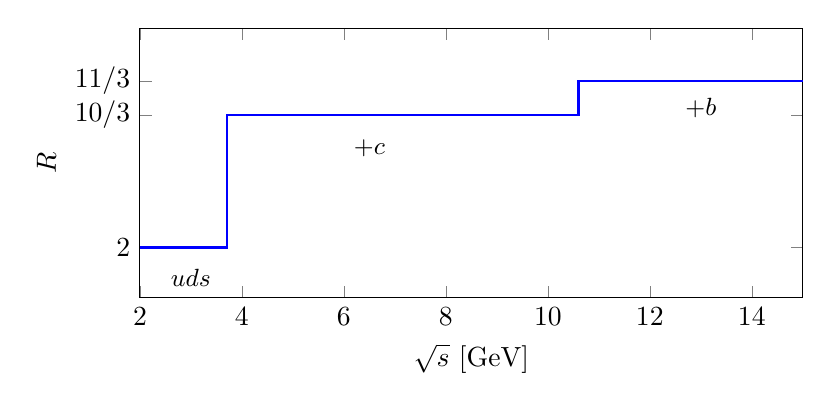
\begin{tikzpicture}
\begin{axis}[width=10cm,height=5cm,xlabel={$\sqrt{s}$ [GeV]},ylabel={$R$},
   xmin=2, xmax=15, ymin=1.5, ymax=4.2, samples=2,domain=2:15,
   ytick={2,3.33,3.67}, yticklabels={$2$,$10/3$,$11/3$}]
\addplot[blue, thick, const plot] coordinates {(2,2) (3.7,3.33) (10.6,3.67) (15,3.67)};
\node[font=\small] at (axis cs:3.0,1.7) {$uds$};
\node[font=\small] at (axis cs:6.5,3.0) {$+c$};
\node[font=\small] at (axis cs:13,3.4) {$+b$};
\end{axis}
\end{tikzpicture}
\end{center}
On top of the staircase one sees narrow resonances: $J/\psi(3097),\psi(2S)$ near charm threshold, and $\Upsilon(9460),\Upsilon(2S),\Upsilon(3S)$ near $b\bar b$ threshold.

\textbf{With $\sigma(e^+e^-\to e^+e^-)$ in the denominator:} no, the Bhabha process has both $s$- and $t$-channel contributions, and the $t$-channel diverges as $\theta\to 0$ (small momentum transfer); the total cross section is dominated by forward scattering and is much larger and shape-different. With $\sigma(e^+e^-\to\tau^+\tau^-)$: at $\sqrt{s}\gg 2 m_\tau\simeq 3.6\GeV$ this has the same $1/E^{2}$ form as $\mu\mu$, and below it the cross section vanishes. So the ratio looks the same as with $\mu\mu$ for $\sqrt{s}\gtrsim 4\GeV$, but at lower $\sqrt{s}$ the denominator becomes phase-space-suppressed and $R$ would diverge / not be defined.

%==================================================================
\section*{2.8 \quad GZK cutoff and $\Delta$ baryons}

\Q{$\gamma+p\to\Delta^+\to p+\pi^0$ in CMB.\\
(a) $\Delta(1232)$ quark contents and charges. (b) Force mediating $\Delta^+\to p\pi^0$, Feynman diagram.\\
(c) GZK threshold for $E_\gamma=0.6\,\mathrm{meV}$. (d) $\sqrt{s}$ in $pp$ collision with stationary target, vs.\ LHC.}

\paragraph{(a)} The four $\Delta(1232)$ states (isospin $I=3/2$):
\begin{center}
\begin{tabular}{@{}lcc@{}}\hline
State & Quark content & Charge\\\hline
$\Delta^{++}$ & $uuu$ & $+2$\\
$\Delta^{+}$  & $uud$ & $+1$\\
$\Delta^{0}$  & $udd$ & $0$\\
$\Delta^{-}$  & $ddd$ & $-1$\\\hline
\end{tabular}
\end{center}

\paragraph{(b)} \textbf{Strong} interaction: the decay is $\Delta^{+}\to p\pi^0$ with width $\Gamma\sim 100\MeV$ corresponding to $\tau\sim 5\times 10^{-24}\mathrm{s}$. Quark-level: a $u\bar u$ pair is created via gluon, the $\bar u$ binds with one of the original $u$'s and the $u$ continues, leading to $p+\pi^0$:
\begin{center}
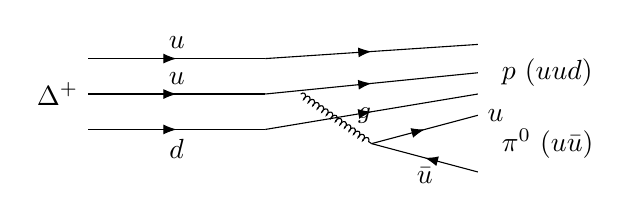
\begin{tikzpicture}[scale=0.9]
\draw[->-=0.5] (-3,1.5) -- (-0.5,1.5) node[midway,above]{$u$};
\draw[->-=0.5] (-3,1.0) -- (-0.5,1.0) node[midway,above]{$u$};
\draw[->-=0.5] (-3,0.5) -- (-0.5,0.5) node[midway,below]{$d$};
\node[left] at (-3,1.0) {$\Delta^{+}$};
% gluon producing u ubar
\draw[decorate, decoration={coil, segment length=2pt, amplitude=1pt}] (0,1.0) -- (1,0.3); \node[font=\small] at (0.9,0.7) {$g$};
\draw[->-=0.5] (1.0,0.3) -- (2.5,0.7) node[right]{$u$};
\draw[->-=0.5] (2.5,-0.1) -- (1.0,0.3) node[midway,below]{$\bar u$};
% Outgoing
\draw[->-=0.5] (-0.5,1.5) -- (2.5,1.7) node[right]{};
\draw[->-=0.5] (-0.5,1.0) -- (2.5,1.3) node[right]{};
\draw[->-=0.5] (-0.5,0.5) -- (2.5,1.0) node[right]{};
\node[right] at (2.7,1.3) {$p$ ($uud$)};
\node[right] at (2.7,0.3) {$\pi^0$ ($u\bar u$)};
\end{tikzpicture}
\end{center}
Vertices are gluon-quark; force = strong (QCD).

\paragraph{(c) GZK threshold.} Threshold (head-on collision) for $\gamma+p\to\Delta^+$ in c.m.\ frame:
\[
s=(p_p+p_\gamma)^{2}=m_p^{2}c^{4}+2 E_p E_\gamma(1-\cos\theta_{p\gamma})\to M_\Delta^{2}c^{4}.
\]
For head-on ($\cos\theta=-1$, photon and proton anti-parallel):
\[
M_\Delta^{2}c^{4}-m_p^{2}c^{4}=4 E_p E_\gamma\Rightarrow E_p=\frac{M_\Delta^{2}-m_p^{2}}{4 E_\gamma}c^{2}.
\]
Numerically: $M_\Delta^{2}-m_p^{2}=1232^{2}-938^{2}=(1232-938)(1232+938)\MeV^{2}=294\cdot 2170=6.38\times 10^{5}\MeV^{2}$. With $E_\gamma=6\times 10^{-10}\MeV$:
\[
E_p^\mathrm{thr}=\frac{6.38\times 10^{5}\MeV^{2}}{4\cdot 6\times 10^{-10}\MeV}=\boxed{\,2.66\times 10^{14}\MeV=2.7\times 10^{20}\,\mathrm{eV}.\,}
\]
(In line with the canonical GZK cutoff $\sim 5\times 10^{19}\,\mathrm{eV}$; using mean photon energy rather than peak gives the slightly higher figure.)

\paragraph{(d)} Such a proton on a stationary terrestrial proton:
\[
s = 2 m_p^{2} c^{4}+2 E_p m_p c^{2}\simeq 2 E_p m_p c^{2}\;\;(E_p\gg m_p),
\]
\[
\sqrt{s}=\sqrt{2 E_p m_p c^{2}}=\sqrt{2\cdot 2.66\times 10^{14}\MeV\cdot 938\MeV}=\sqrt{4.99\times 10^{17}}\MeV
=\boxed{\,7.1\times 10^{8}\MeV=710\,\mathrm{TeV}.\,}
\]
LHC reaches $\sqrt{s}=14\,\mathrm{TeV}$ for $pp$ (Run 3 design), so the GZK proton on a fixed target gives a c.m.\ energy $\sim 50\times$ the LHC. (Equivalently, why fixed-target experiments waste energy and we build colliders.)

\end{document}
